\section{Digital Input}

In this section you will let the outside world talk to the Arduino
and let the Arduino talk to the computer.
The first of these is done by taking a pin and telling the Arduino
to set it aside as an input pin.
The second is done by using the USB cable and telling the Arduino
to print text to it. 
You will also see tristate logic and why buttons will never work
like you expect them to.

You will need the following parts:

\setlength{\tabcolsep}{0pt}
\begin{center}
\begin{tabular}{|c| c |}
\hline
    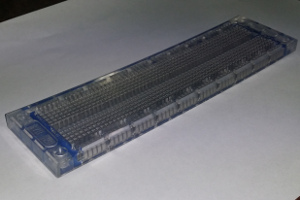
\includegraphics[align=c,width=0.2\textwidth]{./Graphics/breadboard}
    & 
    \begin{minipage}[t]{0.2\textwidth}
        \centering
        1 $\times$ Bread Board 
    \end{minipage}\\ \hline
    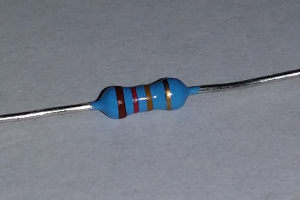
\includegraphics[align=c,width=0.2\textwidth]{./Graphics/12k_resistor} 
    & 1 $\times$ 12K$\Omega$ Resistor \\ \hline
    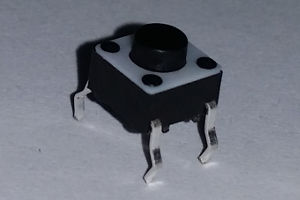
\includegraphics[align=c,width=0.2\textwidth]{./Graphics/push_button}
    & 1 $\times$ Push Button\\ \hline
    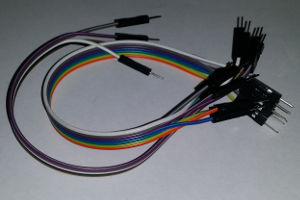
\includegraphics[align=c,width=0.2\textwidth]{./Graphics/jumper_cables}
    & 3 $\times$ Jumper Cables \\ \hline
  \end{tabular}
\end{center}

\subsection{Pull-up Resistor}
Like in the preceding section you will make several circuits
to see the different ways of achieving the same thing.

\begin{center}
    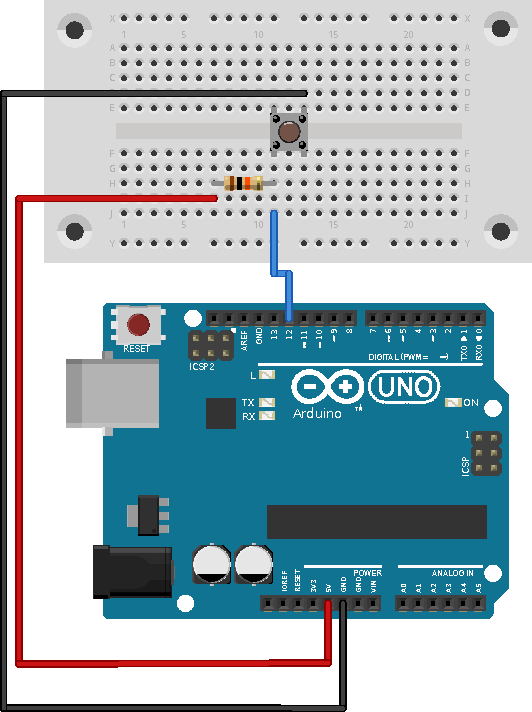
\includegraphics[width=0.4\textwidth]{./Graphics/PullUp}
\end{center}

The first of these is the more ``normal'' circuit.
When the button is not pressed the circuit is ``off''
as you would imagine a switch not being pressed should be.

\begin{center}
    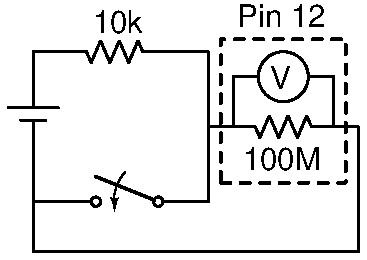
\includegraphics[width=0.3\textwidth]{./Graphics/PullUpCircuit}
\end{center}

The above shows the schematic of the circuit.
Note that the internal resistor has a higher resistance than anything
you have seen so far.


\subsection{Pull-down Resistor}
\begin{center}
    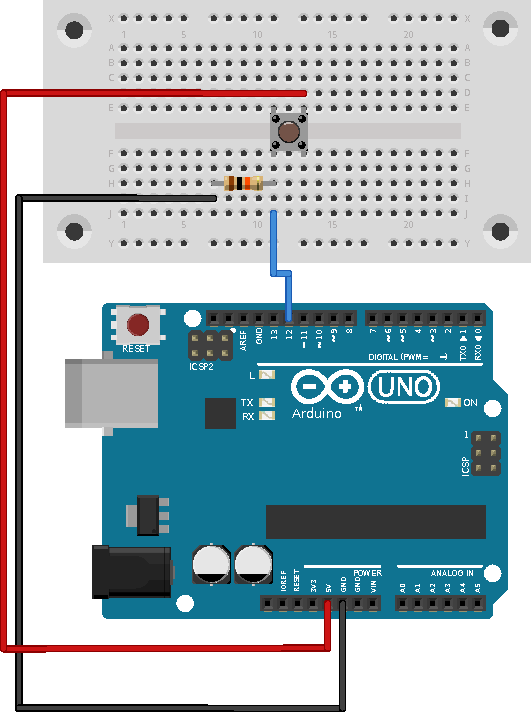
\includegraphics[width=0.4\textwidth]{./Graphics/PullDown}
\end{center}

\begin{center}
    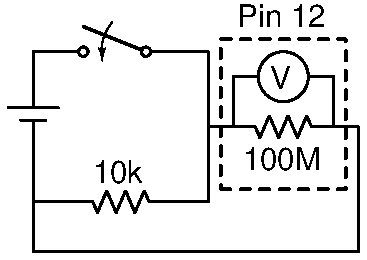
\includegraphics[width=0.3\textwidth]{./Graphics/PullDownCircuit}
\end{center}

\subsection{Tristate Logic}

To understand why you bothered with the weird circuits above
you need know about tristate, or floating logic.
That combined with the demands of building a detector that doesn't disturb the 
circuit during normal operation means you need to ``ground'' all input pins
to stop yourself from having erratic readings.

In the above circuit, for example, if you didn't use one of the pull up or pull down
patterns and just connected the live button to the live wire an input pin
you can get a button pressed even just by hovering your finger over the button
without touching it at all.

Without having at least an acquaintance with it nothing after this will make sense.

\begin{center}
    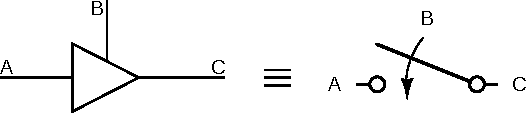
\includegraphics[width=0.4\textwidth]{./Graphics/tristate}
\end{center}



\subsection{Software}
\lstinputlisting[style=Arduino]{./Src/serial.src}

You are using pin 12 here instead of pin 13
because pin 13 has connected to it an LED,
as you learned in the last section an LED causes a voltage drop
of around 2-3V across it,
since the logical ON here is 5V 
this may cause the board to not register a button press.

\subsection{Internal Pulldown}
Because input is so common the Arduino comes with a build in
pull down resistor. 
You can connect the Arduinos output pin and ground directly to the switch.

\begin{center}
    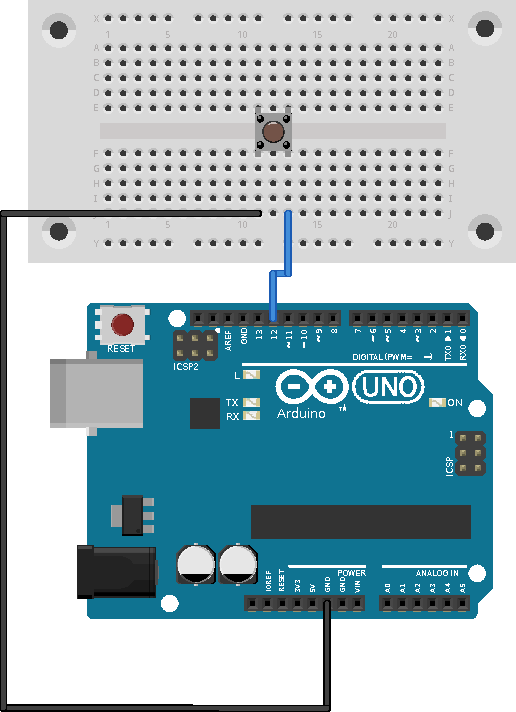
\includegraphics[width=0.4\textwidth]{./Graphics/pull_down_internal}
\end{center}

The internals of the circuit look like:

\begin{center}
    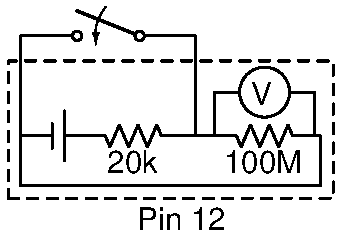
\includegraphics[width=0.3\textwidth]{./Graphics/InternalPullUp}
\end{center}

\lstinputlisting[style=Arduino]{./Src/serial2.src}

Here we see the usefullness of macros, 
\lstinline|HIGH|
keyword here means that we turn on the internall pullup.
\subsection{Hardware}
\begin{center}
    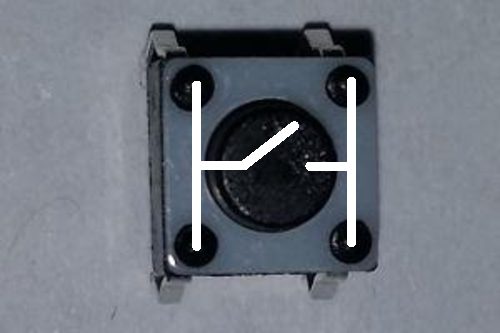
\includegraphics[width=0.2\textwidth]{./Graphics/push_button_internal}
\end{center}

The push button is an instananeous on which stays on so long
as it is pressed.
Note the internal wiring.
